% =====================================================================
% main_mlsys.tex -- MLSys 2027 Research Track target.
%
% Venue re-route per D-063: both TMLR submissions were desk-rejected
% 2026-07-31 and the merged paper was routed here. The 2027 CFP directs
% authors to the mlsys2025 package, which is installed in this directory
% UNMODIFIED. It carries geometry tamper checks (textwidth, textheight,
% margins); altering it is a format violation the venue rejects without
% review. Do not load geometry, fontenc, natbib or fancyhdr here - the
% style file already does, and reloading them is the same violation.
%
% Blind by default: \usepackage[accepted]{mlsys2025} suppresses the author block.
% The camera-ready switches to \usepackage[accepted]{mlsys2025}.
%
% Body and appendices are GENERATED. Run gen_sections.py after any change
% to MERGED_PAPER_v1.0_FROZEN.md; never hand-patch a section file.
% Four-pass build: pdflatex, bibtex, pdflatex, pdflatex.
% =====================================================================
\documentclass{article}

\usepackage{microtype}
\usepackage{amsmath}
\usepackage{graphicx}
\usepackage{booktabs}
\usepackage{longtable}   % Appendix H, 108 rows, one column
\usepackage{hyperref}
\usepackage{url}
% Let long artifact URLs in the bibliography break rather than run into the
% margin. Typesetting only: no geometry is touched and the style file is
% untouched, which is the CG6 T2-h rule.
\Urlmuskip=0mu plus 1mu\relax
\def\UrlBreaks{\do\/\do-\do.\do_\do?\do\&\do=\do:}
\newcommand{\theHalgorithm}{\arabic{algorithm}}

\usepackage[accepted]{mlsys2025}
% READING BUILD: [accepted] drops the review line numbers and the
% "Under review" banner. Not a submission target - main_mlsys.tex is.
% DERIVED from main_mlsys.tex; regenerate rather than hand-edit.

\hypersetup{colorlinks=true, linkcolor=black, citecolor=black, urlcolor=blue}

% The artifact reference is the only content difference between the blind
% and named builds (operator ruling 2026-07-24): under blind review the
% artifact travels WITH the submission as supplementary material, which
% keeps the release inside the double-blind envelope rather than behind a
% third-party proxy that would require a public repository.
\newif\ifanon
\anonfalse
% \ArtifactStatement is the one build-dependent sentence in the paper. It says
% WHERE the release is, and it must precede the Artifacts section's claim that
% nothing reported depends on an unreleased artifact, because that claim is
% only checkable if the reader can find the release.
% ANONYMOUS: no DOI, no URL, no identifier (operator ruling 2026-09-14). The
% CFP rejects anonymisation failures without review, a DOI resolves to a named
% page, and the upside is a check on an artifact reviewers are not required to
% read at a venue whose artifact process runs post-acceptance.
% \ArtifactRepoURL is ALSO consumed by the evalspec2026 bibliography entry, so
% it must be defined in BOTH branches or the bibliography fails to typeset.
% Defining it only in the named branch broke the anonymous build, which is how
% this dependency was found: the macro was never "unused", it was used from the
% .bbl, where a sweep over the generated section files does not look.
\ifanon
  \newcommand{\ArtifactRepoURL}{Supplementary material accompanying this submission}
  \newcommand{\ArtifactStatement}{The release is public and archived under a
    DOI; the identifiers are withheld for anonymous review and are supplied in
    the camera-ready.\ }
\else
  \newcommand{\ArtifactDOI}{\texttt{DOI-PENDING-DEPOSIT}}
  \newcommand{\ArtifactRepoURL}{\url{https://github.com/Sup3rn0vaN0w/mainlabs-reservation-discipline}}
  \newcommand{\ArtifactStatement}{The release is archived under \ArtifactDOI,
    with the working repository at \ArtifactRepoURL.\ }
\fi

\mlsystitlerunning{Reservation-Based Serving for Long-Horizon Agentic Workloads}

\begin{document}

\twocolumn[
\mlsystitle{An Evaluation of Reservation-Based Serving for Long-Horizon
Agentic Workloads}

\begin{mlsysauthorlist}
\mlsysauthor{Sumit P. Ahuja}{ml}
\end{mlsysauthorlist}

\mlsysaffiliation{ml}{Main Labs}

\mlsyscorrespondingauthor{Sumit P. Ahuja}{sumit@mainlabs.ai}

\mlsyskeywords{serving systems, scheduling, agentic workloads,
reservations, pre-registered evaluation}

\vskip 0.3in

\begin{abstract}
We specify a serving-layer discipline for long-horizon agentic
workloads, a completion-oriented resource contract transferring four
lessons packet networking paid for, rationed per-flow guarantees, early
probabilistic class-aware shedding, fate-independent supervision, and
provenance-bound authority, and we evaluate its central economic claim
under a pre-registered protocol: the metric, the kill thresholds, and
the baseline tuning discipline were frozen and committed before any
evaluation system existed, and every subsequent change is a numbered
amendment released with the paper. The claim is that per-flow completion
guarantees, jointly covering compute, a cumulative cross-invocation
token budget, and pinned cache, with a hard non-preemption guarantee,
buy more completed work per provisioned GPU-hour than they strand.
Across 108 cells against six equally tuned baselines at identical
simulated hardware, the answer is no: a median 10.3 percent loss to the
best per-cell baseline, 0 of 108 cells supporting, and the
graceful-degradation hypothesis reversed at the corrected horizon. The
cost is structural: agentic flows idle in tool time at roughly a 5
percent duty cycle, so reserved capacity is stranded at least 88 percent
regardless of configuration, and the deficit peaks exactly at nominal
provisioning. What guarantees buy is also measured: 63.3 to 97.1 percent
interactive tail-latency isolation across most of the region, bounded
containment of runaway flows where the strongest request-oriented
schedulers starve compliant agentic work to zero, and a sign flip in the
mechanism's favor past saturation. The discipline's enforcement
properties, admission where policy binds, a budget that fixes any
runaway's worst case in advance, an audit ledger, and a kill authority
outside the model's reach, were never throughput claims; two are
measured here in the mechanism's favor and the rest hold by
construction. We additionally report a measurement lesson: evaluation
horizons shorter than the workload's flow lifetimes silently corrupt
both completion metrics and baseline tuning, and we give the structural
fix. All code, generators, seeds, manifests, the amendment history, and
the superseded preliminary readouts are released.
\end{abstract}

]

\printAffiliationsAndNotice{}

% body_mlsys.tex -- generated by gen_sections.py. Do not edit.
% MLSys 2027 Research Track; structure ratified at CG2 and
% executed at CG3/CG4. Regenerate, never hand-patch.

\section{Introduction}

Serving systems for large language models schedule work as preemptible
requests. A growing class of workloads arrives in a different shape:
long-horizon agentic flows, units of work with stable identity across
many model invocations, accumulating cache and tool state whose loss
destroys progress, idling between invocations while tools and humans
respond, and delivering value only at completion. This paper specifies a
serving discipline built for such flows, a completion-oriented resource
contract granted at admission, and evaluates it under a specification
frozen before the evaluation system existed, with published thresholds
under which the proposal's central claim dies. The discipline is not
invented from first principles: each element transfers a lesson packet
networking paid for, rationed per-flow guarantees over aggregate
classes, early probabilistic class-aware shedding, fate-independent
supervision, and provenance-bound authority at the edge. One transfer is
deliberately incomplete, since the discipline keys shedding to a ledger
of forward commitments rather than to queue depth, and Appendix D gives
the four lessons in full with the expanded transfer table.

The evaluation begins somewhere unexpected. Under a mixed workload at
moderate overload, the two strongest request-oriented baselines in our
set complete zero compliant agentic flows, scheduling 1 of 107 and
preempting none: admission starvation, not preemption churn. That
failure is also invisible to the audit mechanisms being specified for
agentic systems, because those mechanisms record events and this failure
consists of their absence. Investigating it exposed a measurement
artifact in our own campaign, a horizon shorter than the workload's flow
lifetimes, which right-censors completion metrics and, less obviously,
corrupts baseline tuning. Correcting it changed what the primary
comparison measured.

The corrected comparison kills the proposal. Across 108 pre-registered
cells against six equally tuned baselines at identical simulated
hardware, reservation-based serving loses a median 10.3 percent of
goodput per provisioned GPU-hour and supports the hypothesis in 0 of 108
cells; the secondary graceful-degradation hypothesis is likewise killed,
reversing sign once the horizon was corrected. The cost is structural
rather than configurational. An agentic flow runs a short invocation and
then waits in tool time, a duty cycle of roughly 5 percent by
construction, so reserved capacity is stranded 88 to 95 percent
regardless of configuration, and the deficit peaks exactly at nominal
provisioning where work-conserving schedulers are at their best.

What the guarantees buy is measured rather than argued away: interactive
tail latency improves by 63.3 to 97.1 percent across most of the region,
an isolation operators currently purchase by overprovisioning and that
the discipline prices in stranded capacity instead; runaway flows are
contained to a bounded degradation; and past saturation the sign of the
primary comparison flips. The mechanism's enforcement properties were
never throughput claims, and two of them are measured here: the budget
contains a runaway to a bound fixed at admission, and the distinction
between a priority and a contract shows up as 106 of 107 compliant flows
starved under the former and half completed under the latter. What the
evaluation removes is the ability to sell any of it as free. This paper
contributes: a serving-layer discipline for long-horizon agentic flows,
specified to the depth required to judge its evaluation (Section 3, with
the full specification in Appendix A); the first controlled comparison
of completion-oriented against preemption-oriented scheduling for such
workloads, seven policies on identical hardware with byte-identical
workload realizations per cell under an equal-budget tuning protocol
enforced by test (Sections 4 to 6); a measured starvation result for
request-oriented scheduling under agentic load, with its observability
consequence (Section 6.1); a measurement-methodology finding with a
structural fix, quantified (Section 6.2); and a quantified decomposition
of what completion guarantees cost and what they buy (Sections 6.3 to
6.6). The pre-registration machinery, frozen thresholds, a numbered
amendment log, an input-domain guard on the verdict path, and the
release of every artifact including superseded readouts, is described as
method, because for a paper whose headline is its own proposal's death
the method is the product.

\input{02_flows_not_requests}
\section{The reservation discipline}

The discipline adds one object and one decision to the serving stack. The
object is the reservation: a ledger entry binding a flow to a guaranteed
resource vector for a lifetime. The decision is admission: whether a flow
enters the small reserved subset, enters an aggregate service class, or is
declined early. Everything else in this section is the precise semantics
of those two things, together with the supervisory and trust elements that
complete the contract. We emphasize at the outset what the discipline
keeps: the gateway accounting of Section 2 remains the identity and
metering substrate, and the scheduling engines of Section 2 remain the
execution machinery. The discipline sits at admission and constrains what
those layers may do to an admitted flow; it replaces neither.

A flow arrives with a descriptor: an estimated invocation count, a
requested cumulative output-token budget, an estimated cache footprint, a
service class, and a provenance class. Admission to the reserved subset
requires five conditions jointly, of which the load-bearing ones are that
the subset holds fewer than K flows, that projected commitment over a
forecast window stays under a configured ceiling, and that some device
set can hold the flow's cache footprint under the pinning rules. A flow
failing any condition is served in an aggregate class or declined early,
which is the cheapest moment in a flow's life to say no.

An admitted reservation covers three resources jointly, and the jointness
is the point, because a flow starved on any one of them fails entirely: a
compute share sufficient for its class latency budget, a cumulative
output-token budget metered at decode across every invocation of the
flow, and key-value cache pinned against eviction and migration for the
reservation lifetime, including across the idle gaps between invocations.
The budget is simultaneously a floor and a bound. Budgeted capacity is
committed, so the flow cannot be silently starved out of it, and the flow
cannot exceed it, so a runaway is a contained event rather than a
discovered one. Pinning has two embodiments, strict and tiered, the
latter spilling to a guaranteed restore path between invocations; the
evaluation prices both without favour.

The guarantee is stated negatively, and the reason is a claim about
auditability rather than style: for the reservation lifetime, no
resource-motivated action of the serving stack may preempt the flow's
invocations, evict or migrate its pinned cache, or reclaim its committed
budget. A prohibition can be audited for violations; a permission cannot
be audited for its non-occurrence. The sole override is a halt issued by
the management plane, which is a safety revocation under designated
authority and definitionally not scheduler preemption, since no capacity
condition can trigger it. A guarantee with a capacity-triggered escape
clause is a priority, and priorities are what the schedulers of Section 2
already have.

All other traffic runs in aggregate service classes with latency budgets
and scheduling weights, degraded under pressure by a probabilistic ladder
whose probability is keyed to committed headroom computed from the
reservation ledger rather than to observed queue depth. That keying is a
design claim the evaluation tests directly, not an assumption it rests
on.

Two elements complete the contract and were never economic claims. A
management plane holds pre-authorized halt, steer, and escalate
authority in a failure and trust domain separate from the inference
stack, which yields four properties that hold by construction: admission
is where organizational policy binds to a flow, the budget fixes any
runaway's worst case in advance rather than in an incident review, the
reservation ledger is the audit record, and the halt does not route
through the model being doubted. Two of the four are measured here
rather than asserted: Section 6 reports what the budget does under
adversarial injection, and what the difference between a priority and a
contract costs the flows subject to it. Trust-keyed admission gates
reservation eligibility on the provenance of the content driving a flow,
fixed before that content is interpreted. Appendix A carries the full
specification: the admission test, the ledger invariants, the
budget-exhaustion vocabulary, lease and multi-tenant semantics, and the
survivability embodiment.

\section{Pre-registered design}

The evaluation specification was frozen on 2026-07-06, before any simulator
code existed, and committed to an append-only repository; the frozen text
with its complete amendment log is released with this paper \citep{evalspec2026}.
This section restates its commitments; the specification governs where they
differ.

Primary metric. Task-level goodput per provisioned GPU-hour: value-weighted
completed flows per hour, normalized by provisioned capacity. The
normalization is the honesty mechanism: capacity a reservation holds idle
lowers the discipline's own score arithmetically, so stranding, the
mechanism's known cost, is priced inside the headline number rather than
negotiated beside it. Value weights are fixed in the specification and
varied only in a declared sensitivity sweep. Related serving metrics score
completed requests against latency targets \citep{mars2026}; ours differs in unit
and denominator, flow completions valued per provisioned GPU-hour, so that
held-but-idle guarantees are charged to the discipline that holds them.

Thresholds, fixed before data. Support required a median improvement of at
least 10 percent over the best baseline, selected per cell as the strongest
tuned opponent in that cell (deliberately conservative against the
mechanism), across at least 60 percent of the core region, with
interactive-traffic p95 time-to-first-token degradation held under 5
percent. Below 5 percent median improvement, or on guardrail violation
across the region: kill. Between: a weak result. The verdict is computed
mechanically by released code as a pure function of the run manifests.

Region. The core region spans interactive-to-agentic traffic mixes (90/10,
70/30, 50/50 by token volume), offered loads 0.7 to 1.5 times measured
capacity, idle-gap distributions with medians of 20, 60, and 300 seconds,
and cluster sizes of 8 to 32 devices (Amendment 3, below). Corner cells
were pre-declared excluded; none required exclusion in the final grid.

Baselines and fairness. Six baselines: vLLM-style priority scheduling
with preemption and paged cache \citep{vllm2023}; FastServe-style multi-level
feedback queues \citep{wu2023fastserve}; Niyama-style deadline-aware class
scheduling, implemented here with a deterministic demotion ladder
\citep{niyama2025}; CONCUR-style AIMD admission with pause/resume
\citep{concur2026}; a MARS-style external admission controller with
cost-benefit cache retention \citep{mars2026}, added by Amendment 1; and FCFS
continuous batching as the no-control floor. Every tunable policy,
including ours, received an identical tuning budget: an 8-point
pre-registered grid, tuned per workload family on validation seeds and
scored on disjoint held-out seeds, with a build-failing test asserting
no policy's grid is larger than any other's. Each baseline is a
policy-family abstraction rather than a reimplementation of any single
system: the families are named for the work that characterises them, and
the comparison is against the scheduling discipline each represents. The
tuned parameters and both scores are released (Table~\ref{tab:roster}, in Appendix G).

The registration carries three numbered amendments and one integrity
ruling, each dated, reasoned, and adopted before the final grid ran: a
baseline added because a negative headline makes baseline completeness
load-bearing, a measurement horizon corrected, and the grid's device axis
reduced after measured infeasibility. All were adopted under a one-fix
clause barring any further measurement correction in either direction,
which is why the verdict below stands as computed; Appendix E gives the
log in full.

\section{Simulator and integrity}

The evaluation runs on a discrete-event simulator at invocation granularity
with token-rate service models: cluster of devices with per-device memory,
batch-size-dependent decode throughput, prefill cost, and modeled host
spill; validated against closed form (Little's law holds to 0.00 percent on
a degenerate configuration, utilization tracks offered load within 1
percent, and these sanity numbers remained bit-identical through every
subsequent engine change).

Two design rules carry the comparison's fairness. First, strict
policy/engine separation: the engine owns all physics, what preemption
costs in both recompute and swap variants, how pinning constrains paging,
how budgets are metered at decode, and the physics are identical for every
policy; policies are pure decision modules behind one interface, and the
reservation ledger's invariants (no over-commitment of compute, memory, or
budget under any event interleaving; no capacity condition in any release
path) are engine-enforced hard test failures. Second, paired comparison:
within a cell, every policy runs against byte-identical workload
realizations from shared seeds, verified by test, so cross-policy deltas
are not workload noise.

Service-model constants (single-stream decode rate, peak decode, cache
bytes per token, spill bandwidth) are literature-anchored and marked low
confidence; Section 6.6 reports their measured sensitivity, including which
constants bind in which regimes and why. No hardware phase was run: the
program gated hardware confirmation on this evaluation supporting the
mechanism, and the gate closed.

Three construction defects were caught by the engine's own invariants
before the campaign ran, and one of them was depressing the
work-conserving baselines that go on to win the final comparison, so
leaving it unfixed would have made the mechanism's loss look smaller for
a reason unrelated to scheduling. Two further interventions occurred
during the campaign and are disclosed in the released readouts: 189
pre-amendment manifests were quarantined behind a new input-domain guard,
and two baseline runs that reached congestion collapse were excluded with
their selection effect stated, a bias that favours the affected baselines
and therefore runs against the mechanism this evaluation killed. Appendix
F records all five.

\section{Results}

All numbers are from the final campaign: 2,268 H1 runs over 108 cells at
the Amendment 2 horizon, 252 H2 runs, 84 H3 runs, and 162 ablation runs
over two operating points, with full manifests released. Figures and
tables supporting each result beyond the two carried inline are in
Appendix G, and the full per-cell table is Appendix H. Two baseline runs
reached congestion collapse at the wall-clock cap and are excluded with
their selection effect disclosed in the readout; the exclusion flatters
the affected baselines and therefore runs against the mechanism.

\subsection{Request-oriented schedulers starve agentic flows}

The campaign's first result is not about reservations. Under a mixed
workload at 1.2x offered capacity, the two strongest request-oriented
baselines in the set, vLLM-style priority scheduling with preemption and
Niyama-style deadline-aware class scheduling, complete 0.000 of compliant
agentic flows. Not a degraded fraction: zero, at every level of
adversarial injection including no injection at all (Figure~\ref{fig:containment}).


\begin{figure}[tbp]
\centering
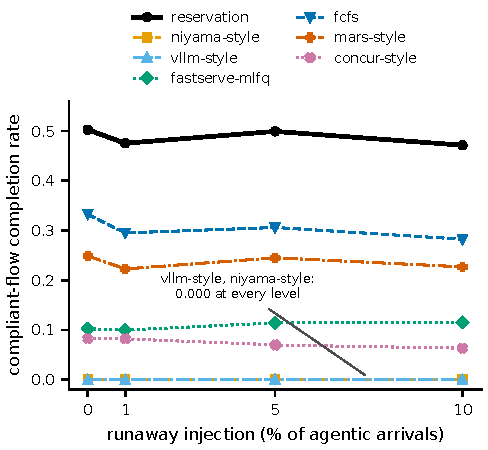
\includegraphics[width=3.25in]{figures/F4_containment_starvation.pdf}
\caption{Compliant-flow completion under adversarial runaway injection, absolute rates. The reservation discipline holds near 0.5 with a worst-case degradation of 3.1 points; FCFS completes 0.33 with no containment; the two strongest request-oriented baselines complete zero compliant flows at every level including no injection, instrumented admission starvation (one of 107 compliant flows ever scheduled, zero preemptions; Section 6.1). Deltas against zero are undefined, which is why rates are absolute.}
\label{fig:containment}
\end{figure}

This is not a missing measurement. Instrumentation of the cell shows
those policies schedule 1 of 107 compliant agentic flows, with zero
preemptions. Under interactive-class priority, long flows never receive a
device slot while interactive traffic saturates the cluster. The failure
is admission starvation rather than preemption churn, and the result is
locked by a regression test. A delta against zero is undefined, which is
why this section reports absolute completion rates throughout.

The starvation is also invisible to the audit mechanisms being specified
for agentic systems, and that consequence is worth stating separately
because it generalizes beyond scheduling. Those mechanisms are
event-based: they record what a flow did, which tools it called, what it
returned. A flow that is admitted, never scheduled, and still live at
the horizon produces no events to record, and a conformant audit trail
for such a flow is an honest and indefinitely long sequence of nothing
having happened. The failure consists of the absence of events, so
event-triggered analysis cannot surface it without a liveness test: the
record is complete, and the fault is invisible inside it.

Against that baseline, the discipline's cross-invocation budget does
what it was specified to do. Compliant-flow completion holds at 0.503,
0.475, 0.499 and 0.471 across injection levels, a worst-case degradation
of 3.1 points, and every runaway is cut off at exactly its budget. FCFS,
blind to class, completes 0.332 and degrades 5.0 points under injection:
no isolation and no containment, but no starvation either. The
discipline is the only policy in the set that is simultaneously above
0.3 absolute and below 3.5 points of adversarial degradation. Section 3
distinguished a priority from a contract as a matter of kind; this is
that distinction as a matter of record. Appendix G tabulates every
policy's rate at every injection level.

\subsection{The horizon lesson}

Investigating those zeros produced the campaign's most generalizable
finding, and it concerns measurement rather than scheduling. The
diagnostic that established the starvation as genuine also showed that
every sweep in the campaign was running a measurement horizon far shorter
than the workload's own timescale.

The median agentic flow requires roughly 711 seconds to complete with no
queueing at all, tool-time gaps plus decode service; the figure was first
measured at roughly 863 seconds on the diagnostic realization that
surfaced the problem, and the released generator derivation, which any
reader can run, gives 711. The build's default horizons ran 150 to 300
seconds, and at a 200-second window only about a quarter of agentic flows
could complete on an idle cluster. The primary metric counts completed
flows. A window shorter than the unit of value does not measure the
metric; it measures truncation.

The bias is not symmetric, and it points at completion-guaranteeing
policies specifically. A reservation pays its stranding cost during the
flow and collects its payoff at completion; a horizon that ends before
completion charges the full cost against zero payoff, the mechanism's
worst case by construction, while policies that never schedule long flows
at all are barely touched. Quantified on one core cell (Figure~\ref{fig:horizon}), the
discipline's deficit against the best baseline was 22.3 percent at a
300-second horizon and 7.8 percent at 1500 seconds, stable through 6000
seconds; at the longest horizon the discipline completed more flows in
absolute terms than its comparator while still losing on value-weighted
goodput, a real loss, but half the reported one.


\begin{figure}[tbp]
\centering
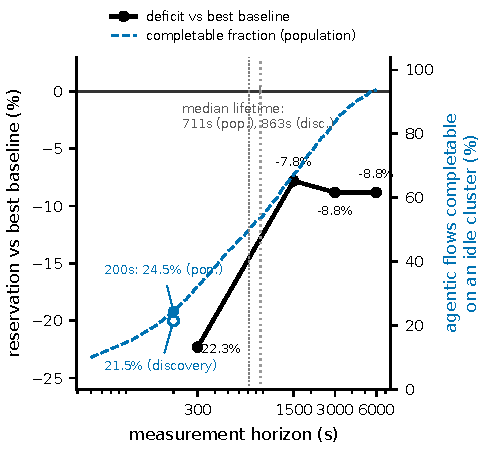
\includegraphics[width=3.25in]{figures/F5_horizon_lesson.pdf}
\caption{Horizon censoring on one core cell. The population median agentic flow lifetime, derived from the released workload generators, is roughly 711 seconds (first measured at 863 seconds on the diagnostic realization that surfaced the artifact, open markers); at a 200-second window only about a quarter of agentic flows can complete even on an idle cluster (24.5 percent of the population; 21.5 percent of the diagnostic realization), while the campaign's default horizons ran 150 to 300 seconds. The measured deficit is 22.3 percent at a 300-second horizon and halves to 7.8 percent at adequate horizons, stable through 6000 seconds. Horizons shorter than the workload's completable lifetimes charge guarantee-holders full stranding cost against zero completion payoff (Section 6.2).}
\label{fig:horizon}
\end{figure}

Censoring corrupts tuning as well as measurement. Re-tuning every policy at the corrected horizon flipped selected parameters across the board, most cleanly for the multi-level feedback baseline, whose chosen quantum moved from the shortest value in its grid to the longest in every workload family: under a censored horizon aggressive demotion looks good because long flows are truncated before their cost lands. An evaluation that had tuned at 300 seconds and measured at 1500 would have compared the mechanism against baselines mis-tuned in its favour. Both tuning campaigns are released, and the fix is structural rather than vigilant: the released code asserts before any sweep runs that the configured horizon exceeds the workload's derivable median flow lifetime, and the verdict path independently rejects any manifest whose horizon disagrees with the grid it claims to report. The correction was adopted as a numbered amendment before the final grid ran, under a one-fix clause barring further measurement changes in either direction, and its full history, including that it improved the mechanism's number on the probe cell and worsened it on the served-value comparison, is in the released amendment log. The rule generalizes to any completion-metric evaluation of long-horizon agents: horizons must exceed the completable-lifetime distribution of the workload, or the benchmark measures its own window. We found the cost of honouring it to be severe, superlinear in the horizon under sustained overload, and it forced a disclosed reduction of our own grid; we suspect the rule is widely violated for exactly that reason.

\subsection{What completion guarantees cost}

Correcting the horizon changed what the primary comparison measured, and
the corrected comparison is the verdict. Computed mechanically against
the frozen thresholds, reservation-based serving loses a median 10.3
percent of goodput per provisioned GPU-hour to the best per-cell tuned
baseline, supports the hypothesis in 0 of 108 cells against a 60 percent
requirement, and holds the interactive guardrail in 96 percent of cells.
Under the specification's thresholds, the hypothesis is killed. The
per-cell improvements are plotted in Appendix G.

The loss has structure worth more than its median. Across offered load
it is U-shaped: at 0.7x capacity the deficit runs 6.6 to 16.1 percent;
at 1.0x it is deepest, 22.4 to 23.6 percent in every cell; at 1.3x it
recovers to 9.5 to 11.5 percent; and at 1.5x the sign flips, with
reservation ahead by 0.8 to 3.2 percent in all 24 non-guardrail-failing
cells. The deficit peaks exactly where the cluster is well-provisioned:
at nominal load the work-conserving baselines run at maximum efficiency
while reservations strand capacity across idle gaps, and as load rises
past saturation the baselines begin to thrash while stranding matters
relatively less, until the ordering inverts at the top of the region.
Completion guarantees, on this evidence, are most expensive precisely
when the fleet is sized correctly.

The other axes are quieter. Cluster size is nearly flat: 8-, 16- and
32-device cells agree within roughly a point throughout, which bears on
the amendment that reduced the device axis, since nothing in the
measured trend suggests the removed 64-device axis behaves categorically
differently. Idle-gap distribution has a mild, consistent effect: longer
gap medians shrink the deficit at low load, because they favour the
tiered-pin embodiment's spill-and-restore over holding hot capacity. At
three seeds the paired bootstrap intervals are tight and solidly
negative in the load 1.0 band, wider at 0.7x where several upper bounds
cross zero. The verdict does not depend on how those intervals are read:
taking every cell at its most favourable bound, 33 of 108 would reach
the support threshold, against the 65 the criterion requires. Both the
cluster-size agreement and the per-cell intervals are read from the full
table in Appendix H.

\subsection{What they buy, and where it inverts}

The guardrail was pre-registered as a constraint, interactive p95
time-to-first-token degraded no more than 5 percent, and the mechanism
did not merely satisfy it: in most of the region it inverted it. At and
above nominal load, reservations improve interactive tail latency by
63.3 to 97.1 percent relative to the best baseline, above 90 percent in
most such cells, while reserved-idle fraction runs 93 to 100 percent in
77 of 81 such cells. Three load-1.5 cells sit at 88.9 percent, admission
having granted few reservations there, and one cell is degenerate at
zero, admission having granted none. Read together with Section 6.3,
this is the ledger's purchase side made precise: the 9.5 to 23.6 percent
goodput deficit buys near-order-of-magnitude tail-latency protection for
interactive traffic, by structurally keeping long flows off the shared
pool. Operators who price interactive tail latency highly are buying
exactly this, and today they buy it by overprovisioning; the discipline
prices the same isolation in stranded capacity instead. Both per-cell
series, tail latency and reserved-idle fraction, are plotted in Appendix
G.

The purchase fails in one measured corner. At heavy agentic mix,
overload, and short gaps, the guardrail fails spectacularly, interactive
p95 time-to-first-token worse by 468.6 to 526.5 percent across all three
cluster sizes. The mechanism is legible: with half the token volume
agentic, gaps short enough that reserved flows cycle almost
continuously, and offered load half again over capacity, the reserved
subset occupies the machine and interactive traffic starves on the
residue. Isolation is a property of the regime rather than of the
mechanism, and it reverses exactly where reservations are densest and
the machine is most oversubscribed. One further isolated failure, at low
agentic mix and nominal load against a FastServe baseline, does not
repeat at any neighbouring cell.

\subsection{Secondary hypotheses and ablations}

The second pre-registered hypothesis held that degradation keyed to
committed headroom yields a better served-value curve under overload
than deterministic demotion and preempt-and-requeue. It does not. Over
the full load sweep from 0.5x to 3.0x, the discipline's served-value
area under curve is 0.626 against the best baseline's 0.648, a 3.4
percent deficit, with two further baselines ahead of it. The comparison
carries only corrected-horizon data: an earlier censored-horizon reading
was ruled unverified and excluded from the released record, and Section
6.2 explains why censored-horizon comparisons mislead. Two baselines
collapse under overload on this metric, both of which protect the system
by throttling intake and pay for it in served value. The full sweep,
with every policy's curve and area, is in Appendix G. One
characterisation requires care. Our implementation of the
deadline-ordered family uses a demotion ladder, while the work it is
named for relegates violating requests to an opportunistic queue rather
than demoting them, so the comparison here is against the deadline
discipline rather than against that system's degradation mechanism. The
distinction does not enter the number: under the equal-budget protocol
the tuner drove that policy's demotion threshold to its maximum in every
workload family, so demotion never fires at the tuned point and the
comparison is effectively against deadline-ordered scheduling with
preemption. A second divergence is not neutralised that way: the
published scheduler interpolates between deadline order and
remaining-work order, while ours orders by class and then deadline
alone.

The ablation campaign removes one element at a time from the tuned
discipline at two operating points: an uncontended nominal-load cell, and
a contended cell with four times the decode slots, elevated load, and the
grid's shortest gaps. Across both, no element shows an effect on the
primary metric distinguishable from seed noise. At the contended cell the
total goodput spread across all nine variants is 0.68 percent against a
within-variant seed spread whose median is 29 percent. One apparent
effect appeared and did not survive: at the nominal cell, replacing
headroom-keyed degradation with queue-depth keying improved goodput by
20.9 percent, but the effect vanished at the contended cell and sits
within the nominal cell's own seed spread; an earlier internal readout
called it corroborating evidence, and that reading is withdrawn in the
released, corrected document. With three seeds a per-element median is a
draw from a distribution wider than the effects being measured, and this
design cannot separate an inert element from an unexercised one. That
noise floor is a property of the ablation design rather than of the
primary comparison: the per-cell deltas of Section 6.3 are paired, every
policy scoring byte-identical workload realizations, which cancels the
workload draw that dominates the unpaired spread here.

What the campaign does establish is robust because it is large and
consistent rather than a difference between near-identical numbers.
Reserved capacity sits 88 to 95 percent idle across both ablation
operating points, a wider and lower band than Section 6.4's because it
includes the contended cell rather than only the at-or-above-nominal
grid cells, despite the contended cell's quadrupled slots, elevated load
and minimal gaps. An agentic flow runs a short invocation and then waits
in tool time, a duty cycle of roughly 5 percent by construction, so
capacity reserved for such flows is stranded nine parts in ten
regardless of configuration. The mechanism's cost is not located in any
single element; it is located in the duty cycle of the workload the
mechanism reserves for. The tuning campaign's independent result points
the same way at larger scale: under the equal-budget protocol the tuner
drove the reserved-subset bound to its grid floor, 5 percent, in every
workload family at both horizons; the tuned-parameter table in Appendix
G shows the corrected-horizon campaign, and both campaigns are released.
Optimized truthfully, the mechanism minimizes itself.

\subsection{Fidelity: what the numbers are conditioned on}

Every number above is conditioned on the simulator's service model, so
the evaluation measured which of that model's constants the result
actually depends on rather than asserting that it does not depend on
them.

One constant binds and it is material. The single-stream decode rate
sets service time: at 0.7x the anchored value, the representative cell's
deficit compresses from 21.5 to 4.4 percent; at 1.3x it is 13.0 percent.
The sign of the verdict is robust across the tested range while the
magnitude is uncertain at roughly the factor the anchor itself is
uncertain. That is the paper's principal fidelity caveat, and it is
unresolvable here because the hardware phase was gated on this
evaluation supporting the mechanism and the gate closed. Appendix G
tabulates the per-constant figures.

Two further constants, peak decode rate and cache bytes per token, do not
move the representative cell's result at all, and the released binding
analysis shows why with instrumentation rather than assertion. At 16
decode slots the batch is capped below the size at which peak decode can
bind, and it was the binding term in 0 of 19,342 decode calls; peak
memory occupancy stays near 39 percent of capacity, so a 30 percent
perturbation changes no placement decision. The same instrumentation was
then run at a deliberately memory-bound configuration, 64 slots with an
agentic-heavy mix at elevated load, where both constants demonstrably
bind: peak decode governs 43 percent of decode calls and memory
saturates. The harness therefore detects binding where binding exists,
and the main grid's device configuration sits in the compute-bound
regime. Regression tests pin all three properties.

\section{Discussion}

The ledger, in one place. Completion guarantees cost a median 10.3
percent of goodput per provisioned GPU-hour in the tested region, and
the cost is U-shaped in load: deepest, 22.4 to 23.6 percent, exactly at
nominal provisioning, recovering toward saturation, inverting past it.
They buy three measured things: interactive tail-latency isolation of
63.3 to 97.1 percent across most of the region, with one identified
inversion corner; containment of adversarial runaways to a 3.1-point
degradation where the strongest request-oriented schedulers starve
compliant agentic work to zero; and a regime boundary at 1.5x load
beyond which the guarantee begins to pay for itself. The efficiency
thesis, that the purchases outweigh the cost on a single
hardware-normalized metric, is dead on its own pre-registered terms.
What survives is a price list.

The honest reading of the mechanism, then, is not ``efficiency technique
that failed'' but ``insurance product whose premium is now known.'' Fleets
that are well-provisioned and run nominal load sit at the bottom of the
U and should not reserve: the premium is maximal there, and the
starvation pathology, while real, is avoidable with cheaper instruments
at low agentic share. The case for reservations concentrates where the
purchases concentrate: fleets that price interactive tail latency highly
and currently buy isolation through overprovisioning; fleets with
adversarial or untrusted agentic exposure, where containment is not
replicable by per-request caps; and fleets that run hot, past
saturation, where the sign has already flipped. Even there, the
K-to-floor result disciplines enthusiasm: reserve for the few flows
whose completion is worth a known premium, and for nothing else, which
is what the rationed-guarantee transfer prescribed before the evaluation
priced it. An operator who prices tail latency or adversarial robustness
as a first-class objective is solving a different optimization, and
Section 6's decomposition is written to let them price it. What cannot
move the verdict is re-measurement under this registration: the one-fix
clause spent its fix, and the number stands.

\section{Limitations}

Simulation only. The hardware phase was pre-gated on this evaluation
supporting the mechanism, and the gate closed; every number here is
conditioned on the simulator's service model. The model's constants are
literature-anchored, marked low confidence, and their measured
sensitivity is the paper's principal caveat: the binding constant moves
the representative deficit between 4.4 and 21.5 percent, sign-stable
throughout. Synthetic workloads: no public traces of long-horizon
agentic serving existed at specification freeze; generators, anchors,
and seeds are released, and the adversarial family is constructed, not
observed. Three seeds per cell (Amendment 3): intervals are wider at low
load, and several 0.7x cells have upper bounds crossing zero
individually, though the verdict is invariant to how they are read,
since taking every cell at its most favourable bound yields 33 of 108
reaching the support threshold against the 65 required. Cluster sizes 8
to 32: the 64-device axis was removed for measured infeasibility at the
corrected horizon; the trend across measured sizes is flat, and the
memory-bound regime is probed at one configuration rather than swept.
Value weights are operator-supplied, fixed at registration, and swept in
sensitivity. H2 and H3 are measured on representative configurations,
not crossed with the full grid. The two-cell ablation design cannot
separate any element's effect from its measured seed-noise floor at
three replications; the campaign attributes the mechanism's cost to the
workload's structural duty cycle, and finer per-element attribution
requires swept axes and more seeds (data released). The comparison also
sets a single completion-oriented policy against six request-oriented
ones, so it prices this contract rather than the class of contracts; a
differently designed completion guarantee is untested here. One boundary
is a non-goal rather than a limitation: this layer enforces decisions
about flows, their admission, their bounds and their termination, and
makes no content-level judgement about what a flow says or does. The
service model does not represent chunked prefill, so one mechanism of
the deadline-ordered family is unmodelled.

Four gaps in the specification were surfaced by readers after the paper
was frozen and are named here rather than quietly repaired. The
discipline specifies when a reservation ends, by expiry, exhaustion,
renegotiation or halt, and never specifies what becomes of the
accumulated pinned state on any of those paths, although Section 3 makes
that state load-bearing. The guarantee is scoped to resource-motivated
action and the halt to safety revocation, so an erasure obligation
arriving from outside the serving stack is neither, and the layer has no
correct move when a reservation lifetime exceeds an erasure deadline.
The disposition vocabulary cannot hold a non-terminating state, yet
Section 6.1 measured one: flows admitted, never scheduled, still live at
the horizon, in none of the four categories. And the workload's idle-gap
distribution is uncertain in both directions at once. Deployments
interposing a human confirmation step, as information-flow control
layers for agents do, carry a tail longer than we modelled, which would
deepen the stranding; production measurement of tool-call latency share
\citep{sutradhara2026} suggests our tool-time anchors may instead be long,
which would shorten it. The sensitivity axis contains no arm below its
own anchor. The verdict is robust to the anchor in either direction,
since Section 6.3 measures that shorter gaps produce larger deficits,
but the attribution of the cost to a roughly 5 percent duty cycle is
conditional on it.

Finally, the
registration's one-fix clause means any residual measurement artifact, in
either direction, stands uncorrected in these numbers by design; the
amendment log is the complete record of what was corrected and when.

\section{Related work}

The serving-layer families were treated in Section 2; here we fix the
distinctions. Four of the six baselines implement the scheduling family
this paper evaluates against directly: priority preemption with paged
cache \citep{vllm2023}, multi-level feedback \citep{wu2023fastserve},
deadline-ordered class scheduling \citep{niyama2025}, and AIMD admission with
pause/resume \citep{concur2026}; migration and chunked-prefill scheduling
\citep{llumnix2024,sarathi2024} are compatible mechanics not separately
evaluated. The MARS-style baseline \citep{mars2026} represents external
admission control for agentic serving; its dynamic SLO goodput is the
nearest metric relative, differing in unit and denominator as Section 4
states, and its cost-benefit cache retention is the advisory counterpart
of the contractual pinning evaluated here, alongside time-to-live and
estimate-driven retention \citep{continuum2025,infercept2024}.
Goodput-oriented routing for agentic inference over heterogeneous pools
\citep{goodserve2026} pursues the same completion-timeliness objective by
placement and migration, within the preemption-family philosophy this
evaluation tests against, and reports gains orthogonal to the admission
question studied here. Program-level schedulers order agentic work
without resource contracts and compose beneath either approach
\citep{autellix2025}; workflow-aware serving \citep{helium2026}, OS-inspired agent
process management \citep{hivemind2026}, and client-side cost-ladder overload
control \citep{unschedulable2026} are likewise compatible and orthogonal.
Gateway budget enforcement \citep{litellm2026,truefoundry2026} supplies the
cumulative accounting the discipline's budgets extend from ceiling to
contract; account-level provisioned throughput \citep{bedrock_ptu,azure_ptu}
reserves at a granularity that cannot see flows, and composes as the
tenant envelope of Appendix A. Batch-system advance reservations,
quality-of-service classes, and gang scheduling \citep{slurm_reservations,k8s_qos,gang_scheduling} are the structural ancestors; what is new here
is what was tested, jointly guaranteed cache-and-budget reservations
across idle gaps at flow granularity, and the finding is that the
ancestors' economics survive the transfer better than the guarantees do.
The network lineage of Section 1 and Appendix D \citep{rfc2205,rfc2475,floyd1993red,rfc2597,rfc2827,rfc3704,ipmi_spec} is inheritance, not
reargued here. Production measurement of tool-based agentic inference
reports tool calls accounting for 30 to 85 percent of end-to-end
first-token latency \citep{sutradhara2026}, a workload shape convergent with
the one modelled here and measured rather than constructed.

Two adjacent literatures bound the discipline's trust and supervision elements, both of which now sit in Appendix A: content-level defences that govern what a piece of content may cause an agent to do \citep{camel2025,fides2025,rtbas2025,wallace2024,pact2026,provgates2026,cxi2026,memcurate2026}, and in-pipeline or execution-time monitoring that supplies verdicts about agent behaviour \citep{llamaguard2023,zou2024circuitbreakers,safetykernel2026,killbench2025}. Both act downstream of admission on content or actions; the discipline's elements act upstream on capacity and standing, and Appendix A states the distinction.
The plane-separation convergence \citep{mozilla2026,dynamo2025,aibrix2025,mars2026} is this paper's premise. On method, pre-registration with
published kill criteria remains rare in systems evaluation; the horizon
result of Section 6.2 relates to right-censoring in survival analysis and
to warmup discipline in queueing simulation, applied to a benchmark
category, completion-metric agent evaluation, that is currently
multiplying.

\section{Conclusion}

This paper proposed a completion-oriented resource contract for the
serving layer, built it from four lessons packet networking paid for,
stated in advance and in public the numbers that would prove its
economics wrong, and then measured them. The economics are wrong: a
median 10.3 percent loss, no supporting cell in 108, the
graceful-degradation hypothesis reversed, and the cause structural, a
workload whose 5 percent duty cycle strands whatever is reserved for
it. What the contract provides regardless, isolation, containment, an
audit record, and a stop that the computation being stopped cannot
reach, is measured or holds by construction, and is now priced rather
than free. The starvation of compliant agentic work by request-oriented
schedulers is no longer an argument but a table. The evaluation leaves
one rule for the benchmarks being built around long-horizon agents: the
horizon must exceed the workload's completable lifetimes, or the
benchmark measures its own window. Every artifact required to check,
retune, or overturn these numbers is released.

\section*{Artifacts}

The release contains: the evaluation specification frozen 2026-07-06
with its complete amendment log and integrity rulings; the simulator
(engine, seven policies behind one interface, workload generators, 141
tests); the tuning harness with both tuning campaigns (censored and
corrected horizons, all tuned parameters and scores); all run manifests
including the quarantined pre-amendment set and the collapsed-run
records; the preliminary readouts with superseded banners intact; the
final readout and the analysis code that computes the verdict as a pure
function of the manifest set; figure-generation code with one command
per figure; and per-figure reproduction commands. \ArtifactStatement Nothing reported in this
paper depends on an unreleased artifact.


\bibliographystyle{mlsys2025}
\bibliography{references}

\appendix
\input{appendix_A}
\onecolumn

\section{Admission test and ledger invariants}

{\small
\begin{verbatim}
State, per pool p: reserved set R_p with bound K_p; capacity vector Cap_p
(compute, device memory, spill-tier memory and restore bandwidth); forecast
window W; committed(p, t) = sum over r in R_p of r's remaining claim
profile over [t, t+W]; per-class budget quotas Q_c; per-tenant envelopes
E_g.

ADMIT(f) for flow f with descriptor (class c, tenant g, budget b, footprint
m, profile est):
  1. |R_p| < K_p
  2. committed(p, t) + claim(est) <= ceiling(p) for all t in window
  3. exists device set D: pinnable(m, D) under embodiment (strict: resident
     throughout; tiered: resident-active plus reserved spill and reserved
     restore within bound L_restore)
  4. spent(c) + b <= Q_c and within E_g
  5. trust(f) >= eligibility threshold for reservation
  All pass: grant r(f), append to ledger, R_p += {f}.
  Any fail: route to class c best-effort, or decline with optional quote.

Events: RENEW is ADMIT at current state with no carried privilege. EXPIRE
and EXHAUST release r(f) with the class's disposition. HALT(authority)
releases r(f) immediately; it is the only release not initiated by the
flow's own lifecycle.

Invariants (any interleaving of admit, renew, expire, exhaust, halt):
  I1 Compute: committed(p, t) <= ceiling(p) <= Cap_p at all t.
  I2 Memory: pinned bytes + reserved spill/restore never exceed their
     tiers; a tiered-pin flow always has a reserved restore path.
  I3 Budget conservation: metered decode tokens of f never exceed b; quota
     accounting is exact under renegotiation.
  I4 Guarantee monotonicity: once granted, r(f) is removed only by expire,
     exhaust, or halt; no capacity condition appears in any release path.
\end{verbatim}
}

\section{The transfer table, expanded}

1. Rationed guarantees. Origin: per-flow reservations failed at scale;
   edge-complexity with core aggregates survived \citep{rfc2205,rfc2475}. Serving
   gap: no per-task guarantee exists at any scale. Element: bounded reserved
   subset K over aggregate classes (Section 4). Leak: K's right size is
   workload-dependent and swept, not derived; the evaluation's tuner chose
   the smallest offered (Section 7.5).
2. Early probabilistic class-aware shedding. Origin: \citep{floyd1993red,rfc2597}.
   Serving gap: deterministic cliffs (demotion at deadline, rejection at
   ceiling). Element: p(H) ladder (Section 4.2). Departure, not transfer: the
   signal is ledger commitments, a forward quantity networks lacked. Leak:
   forecast quality bounds the signal's advantage, and the evaluation found
   no advantage attributable above its noise floor (Sections 7.3, 7.5).
3. Fate-independent supervision. Origin: out-of-band management \citep{ipmi_spec}.
   Serving gap: oversight in the supervised pipeline. Element: management
   plane with authority-and-availability independence (Section 4.3). Leak:
   signal dependence is retained and conceded.
4. Provenance-bound authority at the edge. Origin: ingress source validation
   \citep{rfc2827,rfc3704}. Serving gap: content adjudicated downstream can
   command capacity. Element: trust-keyed reservation eligibility (Section
   4.4). Leak: provenance classes are coarser than network paths, and class
   assignment itself must be trustworthy.

\section{Per-cell H1 results}

Per-cell H1 results, machine-generated from the FINAL readout (cell, best baseline, improvement, 95 percent CI, guardrail; all 108 cells).

{\footnotesize
\begin{longtable}{llrrl}
\toprule
cell & best baseline & improvement & 95\% CI & guardrail \\
\midrule
\endhead
\texttt{mix0.1\_load0.7\_dev16\_gap20.0} & fcfs & -7.8\% & [-7.8\%, +9.6\%] & ok \\
\texttt{mix0.1\_load0.7\_dev16\_gap300.0} & fcfs & -6.9\% & [-6.9\%, +9.1\%] & ok \\
\texttt{mix0.1\_load0.7\_dev16\_gap60.0} & fcfs & -7.3\% & [-7.3\%, +9.3\%] & ok \\
\texttt{mix0.1\_load0.7\_dev32\_gap20.0} & fcfs & -7.3\% & [-7.7\%, +9.9\%] & ok \\
\texttt{mix0.1\_load0.7\_dev32\_gap300.0} & fcfs & -6.6\% & [-6.7\%, +9.2\%] & ok \\
\texttt{mix0.1\_load0.7\_dev32\_gap60.0} & fcfs & -7.0\% & [-7.2\%, +9.5\%] & ok \\
\texttt{mix0.1\_load0.7\_dev8\_gap20.0} & fcfs & -8.5\% & [-8.5\%, +8.5\%] & ok \\
\texttt{mix0.1\_load0.7\_dev8\_gap300.0} & fcfs & -7.8\% & [-7.8\%, +7.9\%] & ok \\
\texttt{mix0.1\_load0.7\_dev8\_gap60.0} & fcfs & -8.1\% & [-8.1\%, +8.0\%] & ok \\
\texttt{mix0.1\_load1.0\_dev16\_gap20.0} & vllm\_style & -23.2\% & [-23.2\%, -3.7\%] & ok \\
\texttt{mix0.1\_load1.0\_dev16\_gap300.0} & vllm\_style & -23.2\% & [-23.2\%, -3.3\%] & ok \\
\texttt{mix0.1\_load1.0\_dev16\_gap60.0} & vllm\_style & -23.2\% & [-23.2\%, -3.6\%] & ok \\
\texttt{mix0.1\_load1.0\_dev32\_gap20.0} & vllm\_style & -23.5\% & [-23.5\%, -4.1\%] & ok \\
\texttt{mix0.1\_load1.0\_dev32\_gap300.0} & vllm\_style & -23.5\% & [-23.5\%, -3.4\%] & ok \\
\texttt{mix0.1\_load1.0\_dev32\_gap60.0} & vllm\_style & -23.5\% & [-23.5\%, -3.6\%] & ok \\
\texttt{mix0.1\_load1.0\_dev8\_gap20.0} & vllm\_style & -22.5\% & [-22.7\%, -3.3\%] & ok \\
\texttt{mix0.1\_load1.0\_dev8\_gap300.0} & fastserve\_mlfq & -22.6\% & [-22.7\%, -5.0\%] & FAIL (+77.2\%) \\
\texttt{mix0.1\_load1.0\_dev8\_gap60.0} & vllm\_style & -22.6\% & [-22.7\%, -3.0\%] & ok \\
\texttt{mix0.1\_load1.3\_dev16\_gap20.0} & niyama\_style & -10.6\% & [-10.9\%, +9.2\%] & ok \\
\texttt{mix0.1\_load1.3\_dev16\_gap300.0} & niyama\_style & -10.7\% & [-11.1\%, +9.5\%] & ok \\
\texttt{mix0.1\_load1.3\_dev16\_gap60.0} & niyama\_style & -10.7\% & [-11.0\%, +9.7\%] & ok \\
\texttt{mix0.1\_load1.3\_dev32\_gap20.0} & niyama\_style & -10.6\% & [-10.7\%, +9.1\%] & ok \\
\texttt{mix0.1\_load1.3\_dev32\_gap300.0} & niyama\_style & -10.8\% & [-10.9\%, +10.1\%] & ok \\
\texttt{mix0.1\_load1.3\_dev32\_gap60.0} & niyama\_style & -10.7\% & [-10.8\%, +9.9\%] & ok \\
\texttt{mix0.1\_load1.3\_dev8\_gap20.0} & niyama\_style & -10.0\% & [-10.7\%, +9.1\%] & ok \\
\texttt{mix0.1\_load1.3\_dev8\_gap300.0} & niyama\_style & -10.2\% & [-10.8\%, +9.2\%] & ok \\
\texttt{mix0.1\_load1.3\_dev8\_gap60.0} & niyama\_style & -10.1\% & [-10.7\%, +8.8\%] & ok \\
\texttt{mix0.1\_load1.5\_dev16\_gap20.0} & niyama\_style & +2.2\% & [+1.5\%, +19.7\%] & ok \\
\texttt{mix0.1\_load1.5\_dev16\_gap300.0} & niyama\_style & +2.0\% & [+1.3\%, +20.3\%] & ok \\
\texttt{mix0.1\_load1.5\_dev16\_gap60.0} & niyama\_style & +2.1\% & [+1.4\%, +20.3\%] & ok \\
\texttt{mix0.1\_load1.5\_dev32\_gap20.0} & niyama\_style & +1.8\% & [+1.6\%, +19.5\%] & ok \\
\texttt{mix0.1\_load1.5\_dev32\_gap300.0} & niyama\_style & +1.7\% & [+1.5\%, +20.5\%] & ok \\
\texttt{mix0.1\_load1.5\_dev32\_gap60.0} & niyama\_style & +1.7\% & [+1.6\%, +20.2\%] & ok \\
\texttt{mix0.1\_load1.5\_dev8\_gap20.0} & niyama\_style & +2.5\% & [+1.9\%, +20.0\%] & ok \\
\texttt{mix0.1\_load1.5\_dev8\_gap300.0} & niyama\_style & +2.3\% & [+1.8\%, +20.9\%] & ok \\
\texttt{mix0.1\_load1.5\_dev8\_gap60.0} & niyama\_style & +2.4\% & [+1.8\%, +20.6\%] & ok \\
\texttt{mix0.3\_load0.7\_dev16\_gap20.0} & fcfs & -10.9\% & [-11.2\%, +10.9\%] & ok \\
\texttt{mix0.3\_load0.7\_dev16\_gap300.0} & fcfs & -7.9\% & [-8.0\%, +9.7\%] & ok \\
\texttt{mix0.3\_load0.7\_dev16\_gap60.0} & fcfs & -9.2\% & [-9.4\%, +10.7\%] & ok \\
\texttt{mix0.3\_load0.7\_dev32\_gap20.0} & fcfs & -10.5\% & [-11.0\%, +11.0\%] & ok \\
\texttt{mix0.3\_load0.7\_dev32\_gap300.0} & fcfs & -7.4\% & [-7.7\%, +9.4\%] & ok \\
\texttt{mix0.3\_load0.7\_dev32\_gap60.0} & fcfs & -8.9\% & [-9.2\%, +10.6\%] & ok \\
\texttt{mix0.3\_load0.7\_dev8\_gap20.0} & fcfs & -11.0\% & [-11.6\%, +10.4\%] & ok \\
\texttt{mix0.3\_load0.7\_dev8\_gap300.0} & fcfs & -8.6\% & [-8.7\%, +8.7\%] & ok \\
\texttt{mix0.3\_load0.7\_dev8\_gap60.0} & fcfs & -9.7\% & [-10.1\%, +10.1\%] & ok \\
\texttt{mix0.3\_load1.0\_dev16\_gap20.0} & vllm\_style & -23.3\% & [-23.3\%, -7.9\%] & ok \\
\texttt{mix0.3\_load1.0\_dev16\_gap300.0} & vllm\_style & -23.3\% & [-23.3\%, -4.1\%] & ok \\
\texttt{mix0.3\_load1.0\_dev16\_gap60.0} & vllm\_style & -23.3\% & [-23.3\%, -5.3\%] & ok \\
\texttt{mix0.3\_load1.0\_dev32\_gap20.0} & vllm\_style & -23.4\% & [-23.5\%, -7.8\%] & ok \\
\texttt{mix0.3\_load1.0\_dev32\_gap300.0} & vllm\_style & -23.5\% & [-23.6\%, -4.6\%] & ok \\
\texttt{mix0.3\_load1.0\_dev32\_gap60.0} & vllm\_style & -23.5\% & [-23.6\%, -5.7\%] & ok \\
\texttt{mix0.3\_load1.0\_dev8\_gap20.0} & vllm\_style & -22.4\% & [-22.9\%, -7.8\%] & ok \\
\texttt{mix0.3\_load1.0\_dev8\_gap300.0} & vllm\_style & -22.4\% & [-22.9\%, -3.9\%] & ok \\
\texttt{mix0.3\_load1.0\_dev8\_gap60.0} & vllm\_style & -22.4\% & [-22.9\%, -5.0\%] & ok \\
\texttt{mix0.3\_load1.3\_dev16\_gap20.0} & niyama\_style & -10.5\% & [-10.8\%, +4.9\%] & ok \\
\texttt{mix0.3\_load1.3\_dev16\_gap300.0} & niyama\_style & -11.0\% & [-11.3\%, +7.0\%] & ok \\
\texttt{mix0.3\_load1.3\_dev16\_gap60.0} & niyama\_style & -10.8\% & [-11.0\%, +6.3\%] & ok \\
\texttt{mix0.3\_load1.3\_dev32\_gap20.0} & niyama\_style & -10.5\% & [-10.7\%, +4.6\%] & ok \\
\texttt{mix0.3\_load1.3\_dev32\_gap300.0} & niyama\_style & -11.1\% & [-11.2\%, +8.2\%] & ok \\
\texttt{mix0.3\_load1.3\_dev32\_gap60.0} & niyama\_style & -10.8\% & [-10.9\%, +7.0\%] & ok \\
\texttt{mix0.3\_load1.3\_dev8\_gap20.0} & niyama\_style & -9.9\% & [-10.5\%, +4.1\%] & ok \\
\texttt{mix0.3\_load1.3\_dev8\_gap300.0} & niyama\_style & -10.4\% & [-11.0\%, +7.1\%] & ok \\
\texttt{mix0.3\_load1.3\_dev8\_gap60.0} & niyama\_style & -10.1\% & [-10.8\%, +5.8\%] & ok \\
\texttt{mix0.3\_load1.5\_dev16\_gap20.0} & niyama\_style & +2.3\% & [+1.8\%, +15.4\%] & ok \\
\texttt{mix0.3\_load1.5\_dev16\_gap300.0} & niyama\_style & +1.7\% & [+1.1\%, +19.1\%] & ok \\
\texttt{mix0.3\_load1.5\_dev16\_gap60.0} & niyama\_style & +2.0\% & [+1.4\%, +17.6\%] & ok \\
\texttt{mix0.3\_load1.5\_dev32\_gap20.0} & niyama\_style & +2.0\% & [+2.0\%, +14.9\%] & ok \\
\texttt{mix0.3\_load1.5\_dev32\_gap300.0} & niyama\_style & +1.4\% & [+1.3\%, +18.9\%] & ok \\
\texttt{mix0.3\_load1.5\_dev32\_gap60.0} & niyama\_style & +1.7\% & [+1.6\%, +17.4\%] & ok \\
\texttt{mix0.3\_load1.5\_dev8\_gap20.0} & niyama\_style & +3.2\% & [+2.1\%, +15.1\%] & ok \\
\texttt{mix0.3\_load1.5\_dev8\_gap300.0} & niyama\_style & +2.6\% & [+1.5\%, +19.1\%] & ok \\
\texttt{mix0.3\_load1.5\_dev8\_gap60.0} & niyama\_style & +2.9\% & [+1.7\%, +17.1\%] & ok \\
\texttt{mix0.5\_load0.7\_dev16\_gap20.0} & fastserve\_mlfq & -16.0\% & [-16.3\%, -5.4\%] & ok \\
\texttt{mix0.5\_load0.7\_dev16\_gap300.0} & fcfs & -9.5\% & [-9.8\%, +10.3\%] & ok \\
\texttt{mix0.5\_load0.7\_dev16\_gap60.0} & vllm\_style & -12.5\% & [-12.9\%, +1.5\%] & ok \\
\texttt{mix0.5\_load0.7\_dev32\_gap20.0} & fastserve\_mlfq & -16.1\% & [-16.3\%, -5.2\%] & ok \\
\texttt{mix0.5\_load0.7\_dev32\_gap300.0} & fcfs & -9.4\% & [-9.4\%, +10.4\%] & ok \\
\texttt{mix0.5\_load0.7\_dev32\_gap60.0} & fcfs & -12.5\% & [-12.5\%, +9.7\%] & ok \\
\texttt{mix0.5\_load0.7\_dev8\_gap20.0} & vllm\_style & -10.0\% & [-15.9\%, -4.7\%] & ok \\
\texttt{mix0.5\_load0.7\_dev8\_gap300.0} & fcfs & -9.8\% & [-9.8\%, +8.8\%] & ok \\
\texttt{mix0.5\_load0.7\_dev8\_gap60.0} & fcfs & -12.8\% & [-12.8\%, +9.2\%] & ok \\
\texttt{mix0.5\_load1.0\_dev16\_gap20.0} & vllm\_style & -22.8\% & [-23.0\%, -13.2\%] & ok \\
\texttt{mix0.5\_load1.0\_dev16\_gap300.0} & vllm\_style & -23.3\% & [-23.5\%, -6.6\%] & ok \\
\texttt{mix0.5\_load1.0\_dev16\_gap60.0} & vllm\_style & -23.2\% & [-23.3\%, -10.1\%] & ok \\
\texttt{mix0.5\_load1.0\_dev32\_gap20.0} & vllm\_style & -23.0\% & [-23.1\%, -13.4\%] & ok \\
\texttt{mix0.5\_load1.0\_dev32\_gap300.0} & vllm\_style & -23.6\% & [-23.7\%, -6.6\%] & ok \\
\texttt{mix0.5\_load1.0\_dev32\_gap60.0} & vllm\_style & -23.4\% & [-23.5\%, -10.0\%] & ok \\
\texttt{mix0.5\_load1.0\_dev8\_gap20.0} & vllm\_style & -22.6\% & [-22.6\%, -13.5\%] & ok \\
\texttt{mix0.5\_load1.0\_dev8\_gap300.0} & vllm\_style & -23.0\% & [-23.0\%, -6.2\%] & ok \\
\texttt{mix0.5\_load1.0\_dev8\_gap60.0} & vllm\_style & -22.9\% & [-22.9\%, -9.3\%] & ok \\
\texttt{mix0.5\_load1.3\_dev16\_gap20.0} & niyama\_style & -10.1\% & [-10.4\%, -2.7\%] & ok \\
\texttt{mix0.5\_load1.3\_dev16\_gap300.0} & niyama\_style & -11.4\% & [-11.6\%, +4.0\%] & ok \\
\texttt{mix0.5\_load1.3\_dev16\_gap60.0} & niyama\_style & -10.8\% & [-11.1\%, +0.8\%] & ok \\
\texttt{mix0.5\_load1.3\_dev32\_gap20.0} & niyama\_style & -10.2\% & [-10.4\%, -2.2\%] & ok \\
\texttt{mix0.5\_load1.3\_dev32\_gap300.0} & niyama\_style & -11.5\% & [-11.7\%, +5.2\%] & ok \\
\texttt{mix0.5\_load1.3\_dev32\_gap60.0} & niyama\_style & -11.0\% & [-11.1\%, +1.5\%] & ok \\
\texttt{mix0.5\_load1.3\_dev8\_gap20.0} & niyama\_style & -9.5\% & [-10.0\%, -3.5\%] & ok \\
\texttt{mix0.5\_load1.3\_dev8\_gap300.0} & niyama\_style & -10.8\% & [-11.4\%, +4.5\%] & ok \\
\texttt{mix0.5\_load1.3\_dev8\_gap60.0} & niyama\_style & -10.3\% & [-10.8\%, +1.0\%] & ok \\
\texttt{mix0.5\_load1.5\_dev16\_gap20.0} & niyama\_style & -1.5\% & [-2.2\%, +6.2\%] & FAIL (+501.7\%) \\
\texttt{mix0.5\_load1.5\_dev16\_gap300.0} & niyama\_style & +1.1\% & [+0.6\%, +15.6\%] & ok \\
\texttt{mix0.5\_load1.5\_dev16\_gap60.0} & niyama\_style & +1.9\% & [+1.2\%, +11.7\%] & ok \\
\texttt{mix0.5\_load1.5\_dev32\_gap20.0} & niyama\_style & -1.4\% & [-1.9\%, +6.9\%] & FAIL (+468.6\%) \\
\texttt{mix0.5\_load1.5\_dev32\_gap300.0} & niyama\_style & +0.8\% & [+0.7\%, +15.9\%] & ok \\
\texttt{mix0.5\_load1.5\_dev32\_gap60.0} & niyama\_style & +1.5\% & [+1.4\%, +11.9\%] & ok \\
\texttt{mix0.5\_load1.5\_dev8\_gap20.0} & niyama\_style & -1.7\% & [-1.9\%, +6.1\%] & FAIL (+526.5\%) \\
\texttt{mix0.5\_load1.5\_dev8\_gap300.0} & niyama\_style & +1.5\% & [+1.0\%, +14.7\%] & ok \\
\texttt{mix0.5\_load1.5\_dev8\_gap60.0} & niyama\_style & +2.2\% & [+1.7\%, +11.5\%] & ok \\
\bottomrule
\end{longtable}

}

\section{Pre-registration: the complete amendment log}

The amendment log, in full. Pre-registration without a change log is
theater; ours has three amendments and one integrity ruling, each numbered,
dated, reasoned, and adopted before the final grid ran. Amendment 1
(2026-07-14): the MARS-style baseline added, because a negative headline
makes baseline completeness load-bearing. Amendment 2 (2026-07-15): all
measurement horizons raised to at least 1500 seconds after a diagnostic
showed the build default (300 seconds) was shorter than the workload's
median flow lifetime (roughly 863 seconds as measured on the diagnostic
realization; the released population derivation gives roughly 711),
right-censoring the large majority of agentic flows (78.5 percent of the
diagnostic realization, roughly 75 percent of the population,
incompletable within a 200-second window) and biasing the primary metric against
reservation-holding policies; adopted with a one-fix clause, no further
measurement correction in either direction, Section 6.2 reports the finding
in full. Amendment 3 (2026-07-20): the device axis reduced to 8/16/32 and
replications to three seeds after direct measurement showed the frozen grid
infeasible at the corrected horizon (projected 39,600 to 49,700 cpu-hours, a single 64-device run
estimated at 24 to 32 wall-clock hours, unparallelizable); direction of effect unknown for the
device axis, neutral for seeds, and the paper states the narrowed scope.
Integrity ruling (2026-07-20): 189 pre-amendment manifests found in the
verdict path's evidence directory were quarantined and an input-domain
guard added that hard-errors on any manifest outside the grid it claims to
report; measurement semantics unchanged.

\section{Simulator integrity record}

Integrity record. We report the evaluation's own caught defects, because
for a negative result the reader's question is whether the loss is real.
Three defects were caught by the engine's invariants during construction,
each fixed and regression-tested, and one of them was flattering the
mechanism: an O(n squared) scheduling path under overload was silently
depressing the work-conserving baselines, the exact policies that win the
final comparison; left unfixed, the mechanism's loss would have looked
smaller for a reason that had nothing to do with scheduling. A second
defect would have violated the tiered-pin restore guarantee; a third let
oversized flows pin most of a device. During the final campaign, two
further interventions occurred, both disclosed in the readout: 189
manifests from a pre-amendment pilot were found in the verdict path's
evidence directory and quarantined behind a new input-domain guard (the
contamination, censored-horizon cells at an excluded cluster size, biased
against the mechanism; it was removed on domain logic, not direction), and
two baseline runs that reached congestion collapse at the wall-clock cap
were excluded with the selection effect stated, a bias that favors the
affected baselines and therefore runs against the mechanism the evaluation
killed. The full test suite (141 tests), the quarantine directory, and the
collapsed-run manifests are released.

\section{Supplementary results and figures}

\begin{figure}[tbp]
\centering
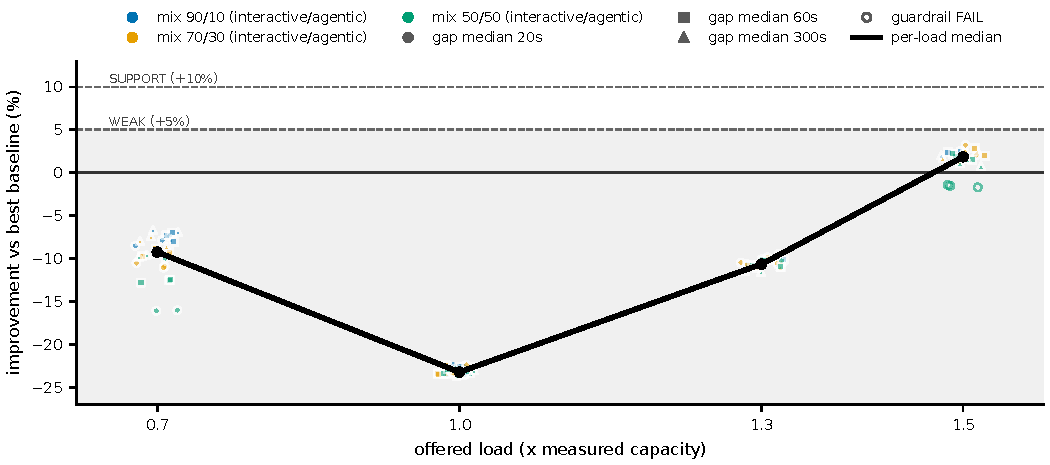
\includegraphics[width=3.25in]{figures/F1_improvement_vs_load.pdf}
\caption{Per-cell improvement of the reservation discipline over the best per-cell tuned baseline, across offered load. Each point is one of 108 pre-registered core cells; the heavy line traces the per-load median. The deficit is U-shaped, deepest at nominal provisioning (22.4 to 23.6 percent at 1.0x), and the sign flips past saturation (+0.8 to +3.2 percent at 1.5x). Dashed lines mark the pre-registered WEAK (+5 percent) and SUPPORT (+10 percent) thresholds; no cell reaches SUPPORT. Open symbols mark the four cells failing the interactive guardrail (Section 6.4).}
\label{fig:improvement}
\end{figure}
\begin{figure}[tbp]
\centering
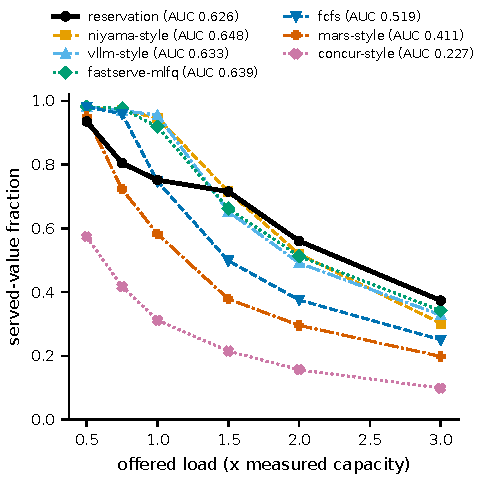
\includegraphics[width=3.25in]{figures/F3_served_value.pdf}
\caption{Served value across the load sweep. The reservation discipline's area under curve (0.626) trails deadline-ordered class scheduling (0.648), killing the graceful-degradation hypothesis; the admission-throttling baselines collapse under overload (Section 6.5).}
\label{fig:servedvalue}
\end{figure}
\begin{figure*}[tbp]
\centering
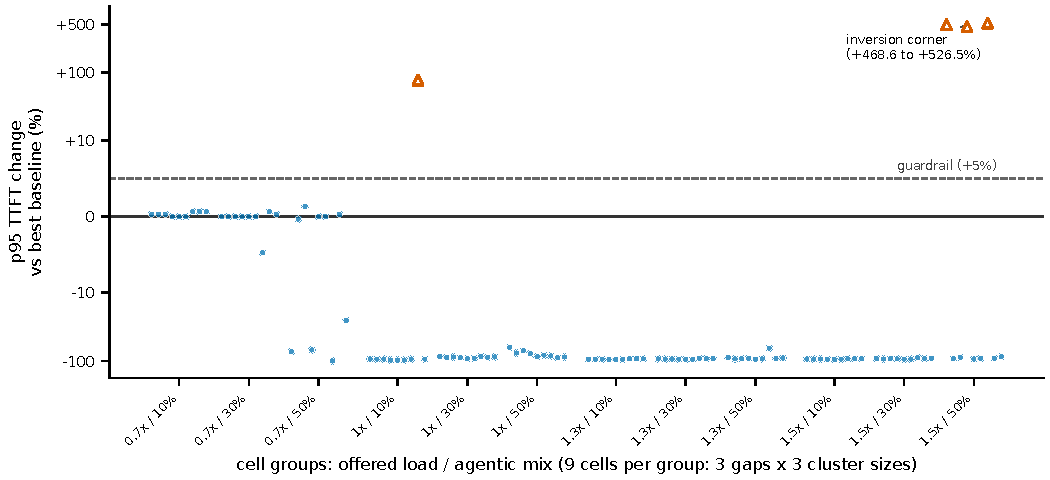
\includegraphics[width=\textwidth]{figures/F2a_interactive_ttft.pdf}
\caption{Interactive tail latency under reservations. Per-cell p95 time-to-first-token change versus the best baseline: at and above nominal load, reservations improve interactive tail latency by 63.3 to 97.1 percent by keeping agentic flows off the shared pool. The effect inverts in the heavy-agentic, overloaded, short-gap corner, where the guardrail fails by 468.6 to 526.5 percent (Section 6.4).}
\label{fig:ttft}
\end{figure*}
\begin{figure}[tbp]
\centering
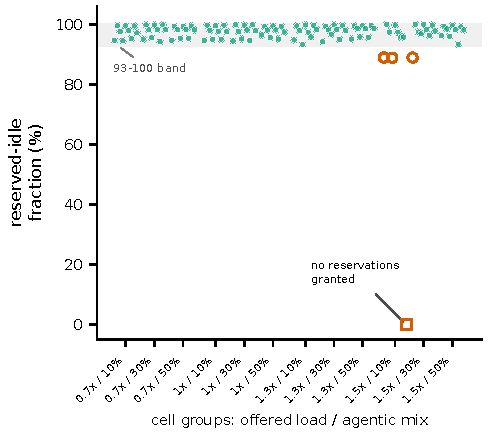
\includegraphics[width=3.25in]{figures/F2b_reserved_idle.pdf}
\caption{What that isolation costs. Reserved-idle fraction per cell: the protection of Figure~\ref{fig:ttft} is priced in capacity held idle, 93 to 100 percent of the reserved pool in 77 of 81 cells, with three load-1.5 cells at 88.9 percent and one cell granted no reservations (marked). This is the structural duty-cycle cost of Section 6.5.}
\label{fig:isolation}
\end{figure}
\begin{table*}[tbp]
\centering
\small
\caption{Policy roster and tuned parameters per workload family (corrected-horizon tuning campaign; 8-point equal-budget grids).}
\label{tab:roster}
\begin{tabular}{llp{4.3in}}
\toprule
policy & workload family & tuned parameters \\
\midrule
concur\_style & mix\_10 & \texttt{additive\_increase=1.0, congestion\_queue\_threshold=0.25, multiplicative\_decrease=0.5} \\
concur\_style & mix\_30 & \texttt{additive\_increase=1.0, congestion\_queue\_threshold=0.25, multiplicative\_decrease=0.5} \\
concur\_style & mix\_50 & \texttt{additive\_increase=1.0, congestion\_queue\_threshold=0.25, multiplicative\_decrease=0.5} \\
fastserve\_mlfq & mix\_10 & \texttt{num\_levels=4, preempt\_mode=swap, quantum\_scale=2.0} \\
fastserve\_mlfq & mix\_30 & \texttt{num\_levels=4, preempt\_mode=swap, quantum\_scale=2.0} \\
fastserve\_mlfq & mix\_50 & \texttt{num\_levels=4, preempt\_mode=swap, quantum\_scale=2.0} \\
fcfs & mix\_10 & \texttt{(no parameters)} \\
fcfs & mix\_30 & \texttt{(no parameters)} \\
fcfs & mix\_50 & \texttt{(no parameters)} \\
mars\_style & mix\_10 & \texttt{additive\_increase=2.0, multiplicative\_decrease=0.75, retain\_threshold\_tokens=500} \\
mars\_style & mix\_30 & \texttt{additive\_increase=2.0, multiplicative\_decrease=0.75, retain\_threshold\_tokens=500} \\
mars\_style & mix\_50 & \texttt{additive\_increase=2.0, multiplicative\_decrease=0.5, retain\_threshold\_tokens=500} \\
niyama\_style & mix\_10 & \texttt{demote\_after\_fraction=1.0, preempt\_mode=swap} \\
niyama\_style & mix\_30 & \texttt{demote\_after\_fraction=1.0, preempt\_mode=swap} \\
niyama\_style & mix\_50 & \texttt{demote\_after\_fraction=1.0, preempt\_mode=swap} \\
reservation & mix\_10 & \texttt{degradation.action=shorten, pin\_mode=tiered, reserved\_subset\_fraction=0.05} \\
reservation & mix\_30 & \texttt{degradation.action=shorten, pin\_mode=tiered, reserved\_subset\_fraction=0.05} \\
reservation & mix\_50 & \texttt{degradation.action=shorten, pin\_mode=strict, reserved\_subset\_fraction=0.05} \\
vllm\_style & mix\_10 & \texttt{max\_batch\_fraction=1.0, preempt\_mode=swap} \\
vllm\_style & mix\_30 & \texttt{max\_batch\_fraction=1.0, preempt\_mode=swap} \\
vllm\_style & mix\_50 & \texttt{max\_batch\_fraction=1.0, preempt\_mode=swap} \\
\bottomrule
\end{tabular}

\end{table*}
\begin{table*}[tbp]
\centering
\small
\caption{Pre-registered verdict summary (thresholds fixed 2026-07-06).}
\label{tab:verdict}
\begin{tabular}{llll}
\toprule
threshold & required & measured & outcome \\
\midrule
median improvement & $\geq$ +10\% (support) / $\geq$ +5\% (weak) & -10.3\% & KILL \\
supporting cells & $\geq$ 60\% of core cells & 0 of 108 (0\%) & KILL \\
interactive guardrail & p95 TTFT degradation $\leq$ 5\% & intact in 96\% of cells & holds (4 cells fail) \\
\bottomrule
\end{tabular}

\end{table*}
\begin{table*}[tbp]
\centering
\footnotesize
\caption{H3 absolute compliant-flow completion rates at each runaway-injection level, with the worst delta versus the no-injection condition (percentage points).}
\label{tab:h3}
\begin{tabular}{lrrrrr}
\toprule
policy & inj 0\% & inj 1\% & inj 5\% & inj 10\% & worst delta \\
\midrule
reservation & 0.503 & 0.475 & 0.499 & 0.471 & -3.1 \\
fcfs & 0.332 & 0.295 & 0.306 & 0.282 & -5.0 \\
mars\_style & 0.249 & 0.223 & 0.245 & 0.227 & -2.6 \\
fastserve\_mlfq & 0.102 & 0.100 & 0.114 & 0.116 & -0.3 \\
concur\_style & 0.082 & 0.082 & 0.070 & 0.063 & -1.9 \\
vllm\_style & 0.000 & 0.000 & 0.000 & 0.000 & +0.0 \\
niyama\_style & 0.000 & 0.000 & 0.000 & 0.000 & +0.0 \\
\bottomrule
\end{tabular}

\end{table*}
\begin{table*}[tbp]
\centering
\footnotesize
\caption{Service-model sensitivity: measured effect and binding classification per constant.}
\label{tab:sens}
\begin{tabular}{llll}
\toprule
constant & perturbation & representative-cell delta & binding \\
\midrule
single-stream decode rate & 0.7x / 1.3x & deficit 21.5\% $\to$ 4.4\% / 13.0\% & binding \\
peak decode rate & $\pm$30\% & none (0 of 19{,}342 decode calls bound) & non-binding \\
cache bytes per token & $\pm$30\% & none (peak HBM near 39\% of capacity) & non-binding \\
\bottomrule
\end{tabular}

\end{table*}

\clearpage

\input{appendix_H}


\end{document}
